% This is samplepaper.tex, a sample chapter demonstrating the
% LLNCS macro package for Springer Computer Science proceedings;
% Version 2.20 of 2017/10/04
%
\documentclass[runningheads]{llncs}
\renewcommand{\baselinestretch}{1.1} 
%
\usepackage{graphicx}
\usepackage[table]{xcolor}
\usepackage{xspace}
\usepackage{hyperref}
\usepackage{subcaption}
\usepackage{listings}
\usepackage{ulem}

\usepackage[para,online,flushleft]{threeparttable}
\usepackage{booktabs}
\usepackage{multirow}
% \usepackage{geometry}
% \usepackage{marginnote}

% Fix link colors
\hypersetup{
    colorlinks = true,
    linkcolor=red,
    citecolor=red,
    urlcolor=blue,
    linktocpage % so that page numbers are clickable in toc
}

% Used for displaying a sample figure. If possible, figure files should
% be included in EPS format.
%
% If you use the hyperref package, please uncomment the following line
% to display URLs in blue roman font according to Springer's eBook style:
% \renewcommand\UrlFont{\color{blue}\rmfamily}
\newcommand{\TG}[1]{\noindent{\color{blue}[\textsc{From Tristan:} #1]}\xspace}
\newcommand{\Ali}[1]{\noindent{\color{green}[\textsc{From Ali:} #1]}\xspace}
\newcommand{\GK}[1]{\noindent{\color{purple}[\textsc{From Greg:} #1]}\xspace}
\newcommand{\YC}[1]{\noindent{\color{orange}[\textsc{From Yohan:} #1]}\xspace}
\newcommand{\anonymous}[1]{***\xspace}


\lstdefinestyle{customC}{
  belowcaptionskip=1\baselineskip,
  breaklines=true,
  xleftmargin=\parindent,
  language=C,
  showstringspaces=false,
  basicstyle=\scriptsize\ttfamily,
  keywordstyle=\bfseries\color[rgb]{0.580, 0.000, 0.827},
  %{purple!40!lightgray},
  commentstyle=\textit{\color{green!40!black}},
  identifierstyle=\bfseries\color{cyan!75!black},
  stringstyle=\color{orange},
  deletekeywords={double,float},
  classoffset=1, % starting new class
  otherkeywords={double,float},
  morekeywords={double,float},
  keywordstyle=\bfseries\color{green!55!black},
  classoffset=0
}

\begin{document}

\title{Comparing tool variability and numerical variability in fMRI analyses}

\author{Ali Salari$^1$, Co-authors$^2$, Tristan Glatard$^1$}

\authorrunning{Salari et al.}
% First names are abbreviated in the running head.
% If there are more than two authors, 'et al.' is used.

\institute{$^1$ Anonymous Organization1\\
  $^2$ Anonymous Organization2\\ **@******.***}

\institute{$^1$ Department of Computer Science and Software Engineering, Concordia University\\
  $^2$ Co-authors Organization\\  Montréal, QC, Canada}

\maketitle              % typeset the header of the contribution

\begin{abstract}
abstract\dots

%  \keywords{Computational reproducibility  \and Neuroimaging pipelines \and Monte-Carlo arithmetic.}
\end{abstract}


\section{Introduction}

\begin{description}
  \item[$\bullet$ ] Methodological choice can influence the final determining areas of brain activation. This opens so results flexibility~\cite{bowring2019exploring}. 

  \item[$\bullet$ ] We presented a framework that can investigate the numerical instability of the pipelines based on Monte-Carlo arithmetic
                    by creating a Fuzzy environment, so that instrument mathematical functions implemented in mathematical system libraries (libmath). 

  \item[$\bullet$ ] In this paper, we aim to answer the questions 1) how the fMRI analyses are numerically stable?
                    2) how the numerical variability is in comparison with the tool variability?
\end{description} 


\section{Methodology}

\subsection{libmath Fuzzy System}

\begin{description}
  \item[$\bullet$ ] libmath Fuzzy allows you to study the numerical stability of tools and pipelines. 
  \item[$\bullet$ ] It is based on MCA perturbations so that applies slight noise on floating-point operations.
  \item[$\bullet$ ] It does not need source code modification or recompilation, and simply works using the Linux LD\_PRELOAD environment variable.
  \item[$\bullet$ ] The library call interposition technique enables us to assess the tools that are dynamically linked to the mathematical library.
\end{description} 


\subsection{fMRI analyses \& Dataset}

\begin{description}
  \item[$\bullet$ ] We replicate the fMRI analyses used in~\cite{bowring2019exploring} using the three most popular packages 
                    for fMRI data processing including FSL, AFNI, and SPM. 
                    
  \item[$\bullet$ ] The functional fMRI studies have been chosen for reanalysis with the publicly available data repositories.
                    The used dataset is available at https://openneuro.org/datasets/ds000001.

  \item[$\bullet$ ] For the ds000001 study, 16 healthy adult subjects participated in a balloon analogue risk task over three scanning sessions.
                    This analysis consists of several common processes. A full description of each analysis is included in~\cite{bowring2019exploring}.

  \item[$\bullet$ ] In the original study, a number of preprocessing steps such as motion correction, segmentation, brain extraction, and registration 
                    were applied in all of the analyses to ensure that results from each software package could be compared objectively.
  
\end{description}  


\subsection{Data processing}

\begin{description}
  \item[$\bullet$ Containerization] building Docker images for three of the most popular software packages in neuroimaging including FSL, AFNI, and SPM.
                  We ensured that the software versions and all the requisites for running analyses used in all experiments 
                  are identical to the original study.  

  \item[$\bullet$ Between tool variability] check and confirm that obtained results are perfectly replicated comparing to the original study. 

  \item[$\bullet$ Numerical variability] running 3 MCA samples in each condition using the Fuzzy libmath environment. 
                  The conditions could be varying between tools, software versions, or the instrumented precisions. 
    \begin{description}
      \item[$\ast$ Varying precisions] a) only perturbing maximum precisions (OS-level), p=53 bits for double-precision and p=24 bits for single-precision.
                                       This would help to compare uncertainty between tool variability and numerical instability at the OS-level. 
                                       b) perturbing precisions from p=53 bits to p=1 bits by steps of 2 iteratively. 
                                       This would help to find the most similar uncertainty distribution between tool variability and numerical variability.
    \end{description}
    
  \item[$\bullet$ Image types] the fMRI result images that we are investigating are thresholded and unthresholded of the group level activation maps.

  \item[$\bullet$ Comparison metrics] comparing variabilities statistically by computing correlations between T-statistic values, Dice coefficient, 
                  and the number of significant digits.    
% EC is a means to assess whether only superficial scaling differences (differences by a scale factor over all voxels) 
% are responsible for disparities between pair of images.

  \item[$\bullet$ Configuration table] showing the detail of the configurations used for replicating the fMRI results.
\end{description}


\section{Results}


% \subsection{Comparing between tool and numerical variability}
\begin{description}
  \item[$\bullet$ Table 1: Summary of statistics] mean and standard deviation of the differences, and correlations 
                  between t-statistic values for each pair of results in each condition.

  \item[$\bullet$ Figure 1 and 2: Surface maps of std.] comparing standard deviations on surface map template (ICBM-152)
                  computed between pair of software (tool variation), and different Fuzzy samples on each software (numerical variation).
                  Figure 1 shows results for group level thresholded t-statistics, and 
                  Figure 2 shows maps for group level unthresholded t values. The numerical variation 

  \item[$\bullet$ Figure 3 and 4: Dice Coefficients] comparing region-by-region Dice coefficients of group level thresholded maps between tools.
                  This measures the overlap of voxels which assess the spatial similarity between activated maps.
                  In bewteen tool similarity, the Dice values correspond to the mean of Dices computed for each pair of that specific tool,
                  for example, Dice value for SPM is calculated by averaging Dices in SPM-AFNI and SPM-FSL pairs.
                  Similarly, Dice values are computed between three Fuzzy samples obtained from each tool in numerical variation.
                  Figure 3 shows bar plots of Dices for negative and positive activated regions.
                  Figure 4 shows surface maps of Dices for the activated regions.

  % \item[$\bullet$ Figure 2: Bland-Altman] comparing unthresholded group level maps, 2D histogram, computed each pair of tools in both conditions.
  % Measures similarity between statistic values.
  % This plots difference between the statistic values (y-axis) and the mean statistic value (x-axis) for all voxels.

  % \item[$\bullet$ Figure 4: Significant digits] comparing the distribution of SD across 3 samples (unthresholded images) for each condition. 
  %                 Find and show results at the precision that creates the most similar numerical uncertainty with between tool variability.  

\end{description}


%%%%%%%%%% Summary of statstics %%%%%%%%
\setlength{\tabcolsep}{10pt}
\begin{table}[h]
    \centering
    \begin{tabular}{cccc|ccc}
        \toprule
        \multirow{2}{*}{} & \multicolumn{3}{c}{Thresholded} & \multicolumn{3}{c}{Unthresholded} \\
        \cmidrule{2-4} \cmidrule{5-7} \\
        {} & Mean diff. & Std. diff. & Corr. & Mean diff. & Std. diff. & Corr.  \\
        \midrule
        \rowcolor{lightgray}
        FSL vs. SPM          &  0.00       & 0.00      & 0.00       & 0.00     & 0.00       & 0.00 \\
        \rowcolor{lightgray}
        FSL vs. AFNI         &  0.00       & 0.00      & 0.00       & 0.00     & 0.00       & 0.00 \\
        \rowcolor{lightgray}
        AFNI vs. SPM         &  0.00       & 0.00      & 0.00       & 0.00     & 0.00       & 0.00 \\
        Fuzzy SPM            &  0.00       & 0.00      & 0.00       & 0.00     & 0.00       & 0.00 \\
        Fuzzy FSL            &  0.00       & 0.00      & 0.00       & 0.00     & 0.00       & 0.00 \\
        Fuzzy AFNI           &  0.00       & 0.00      & 0.00       & 0.00     & 0.00       & 0.00 \\
        \bottomrule
    \end{tabular}
    \caption{Summary of t-statistics mean and standard deviation of differences and correlations of each pair of tools.}
    \label{table:pipeline-stats}
\end{table}


%%%%%%%%%% STD. of Thresh %%%%%%%%
\begin{figure}[b]
  \fbox{\begin{minipage}{\dimexpr \textwidth-2\fboxsep-2\fboxrule}
  \begin{subfigure}[t]{\linewidth}
    \centering
    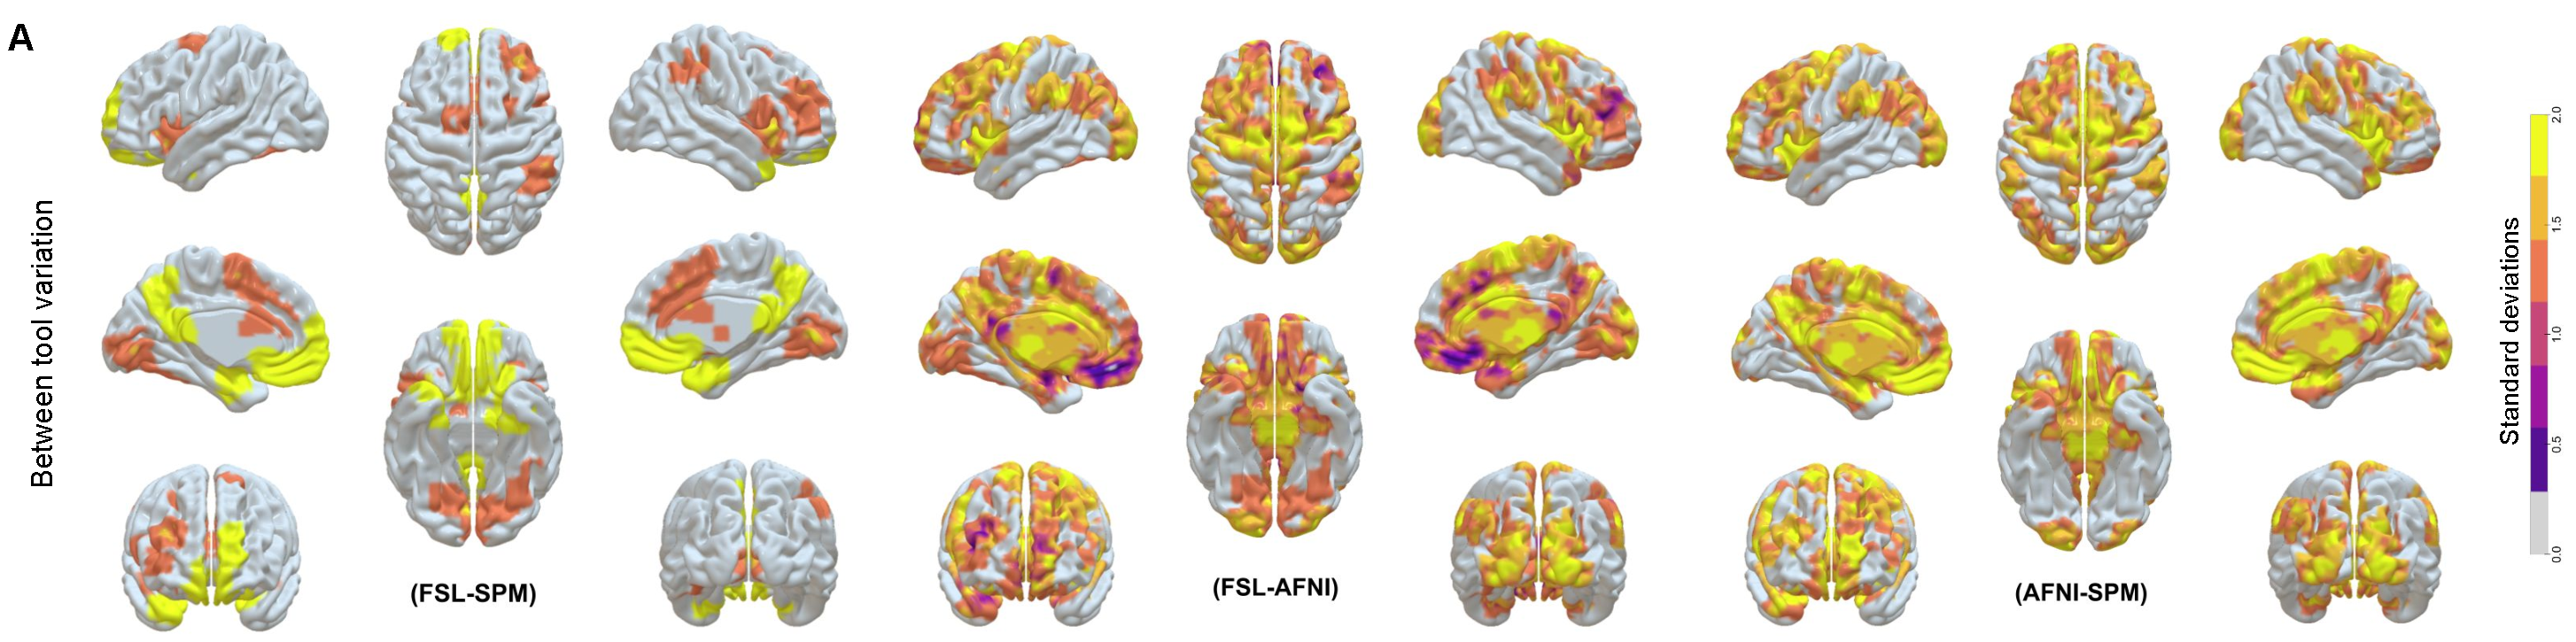
\includegraphics[width=\linewidth]{figures/maps-on-surf-thresh(std).pdf}
    %\caption{Standard deviation of thresholded t-statistics map on template surface}
    \label{fig:thresh-stdmaps1}
  \end{subfigure}
  \hfill
  \begin{subfigure}[t]{\linewidth}
    \centering
    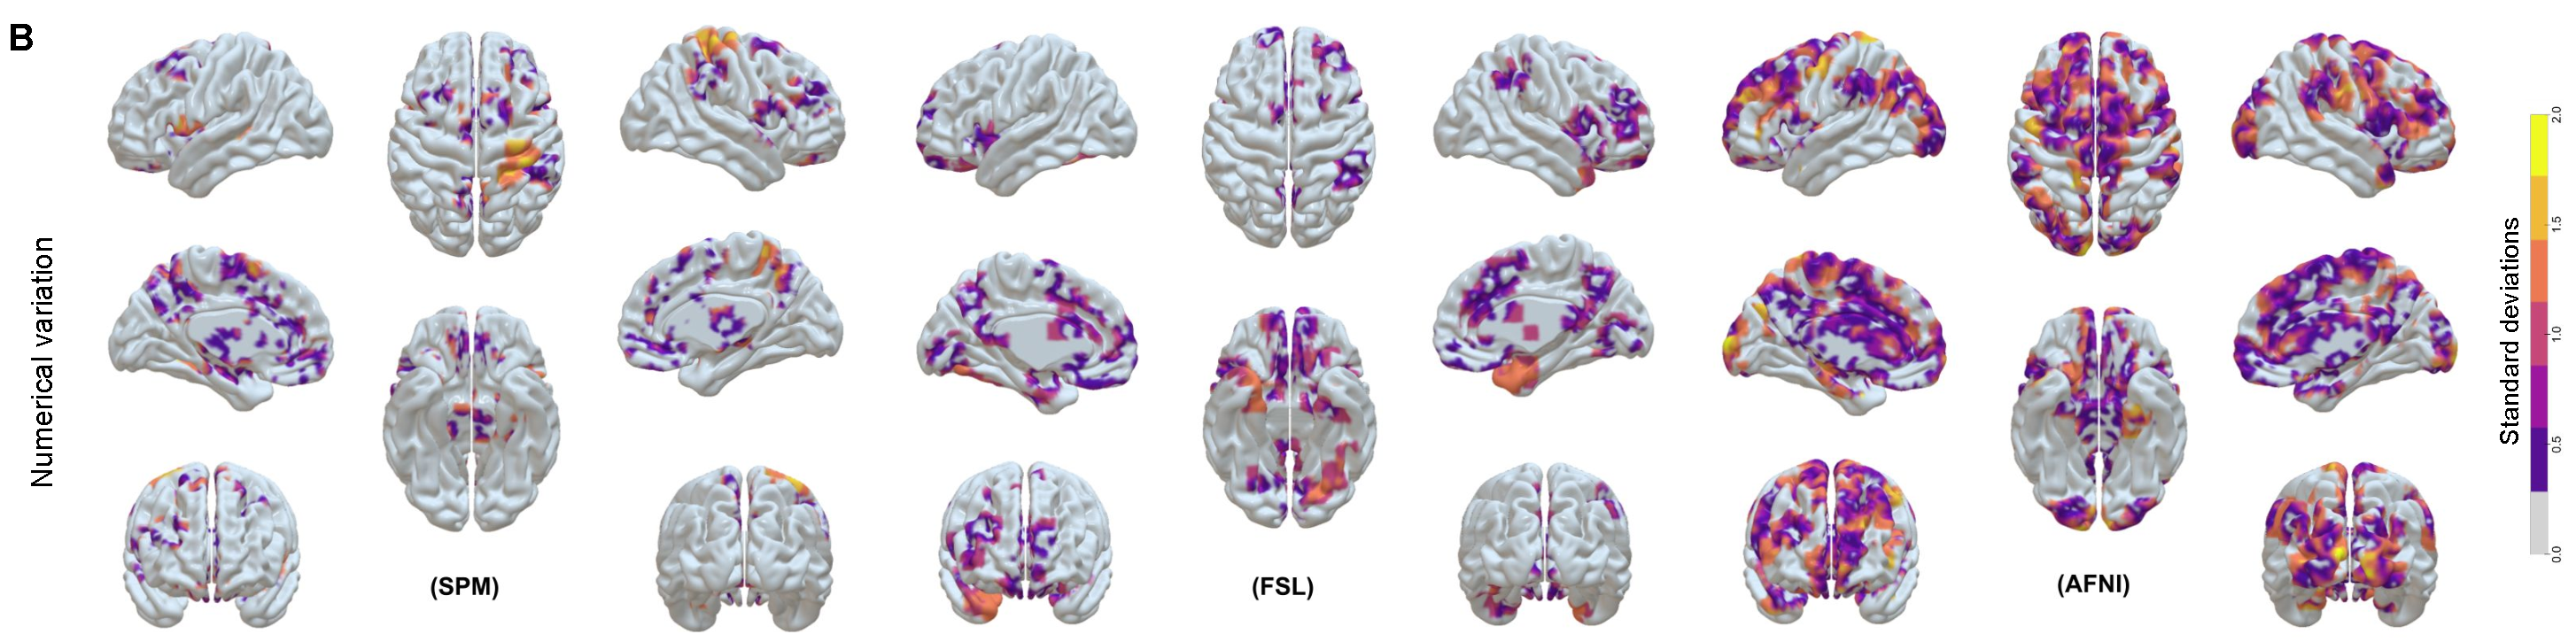
\includegraphics[width=\linewidth]{figures/maps-on-surf-mca-thresh(std).pdf}
    %\caption{Standard deviation of thresholded t-statistics map on template surface}
    \label{fig:thresh-stdmaps2}
  \end{subfigure}
  \caption{Surface maps of standard deviation of thresholded t-statistics.}
  \label{fig:thresh-stdmaps}
  \end{minipage}}
\end{figure}

%%%%%%%%%% STD. of Unthresh %%%%%%%%
\begin{figure}[b]
  \fbox{\begin{minipage}{\dimexpr \textwidth-2\fboxsep-2\fboxrule}
  \begin{subfigure}[t]{\linewidth}
    \centering
    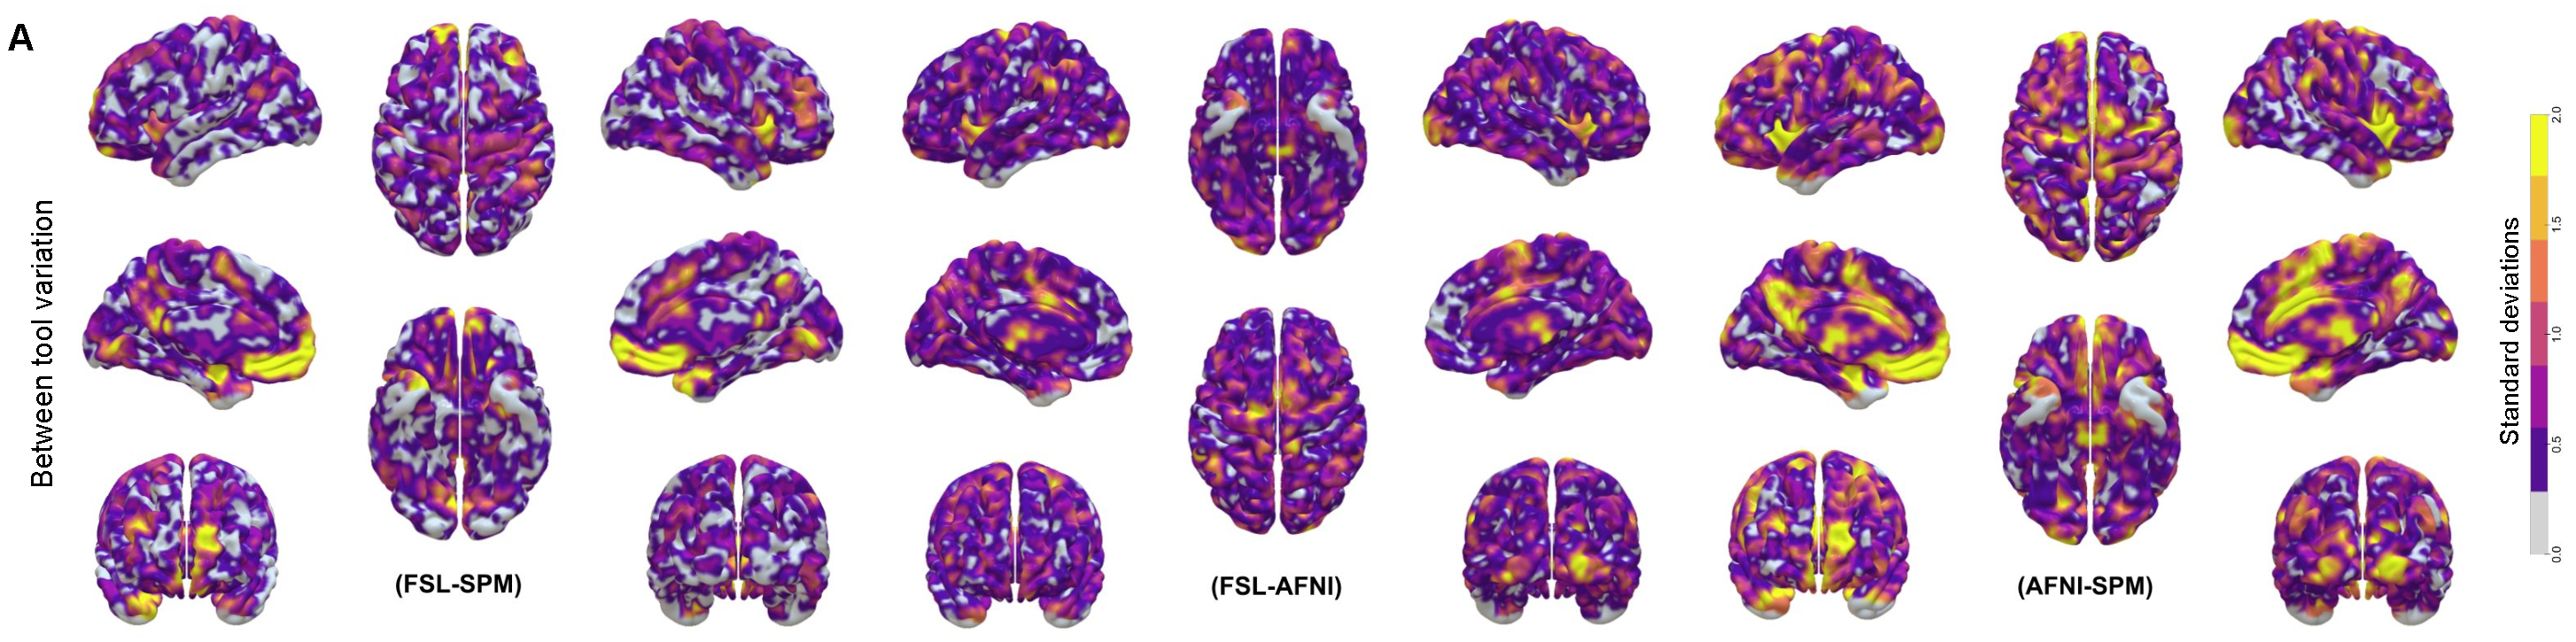
\includegraphics[width=\linewidth]{figures/maps-on-surf-unthresh-tool(std).pdf}
    %\caption{Standard deviation of thresholded t-statistics map on template surface}
    \label{fig:thresh-stdmaps1}
  \end{subfigure}
  \hfill
  \begin{subfigure}[t]{\linewidth}
    \centering
    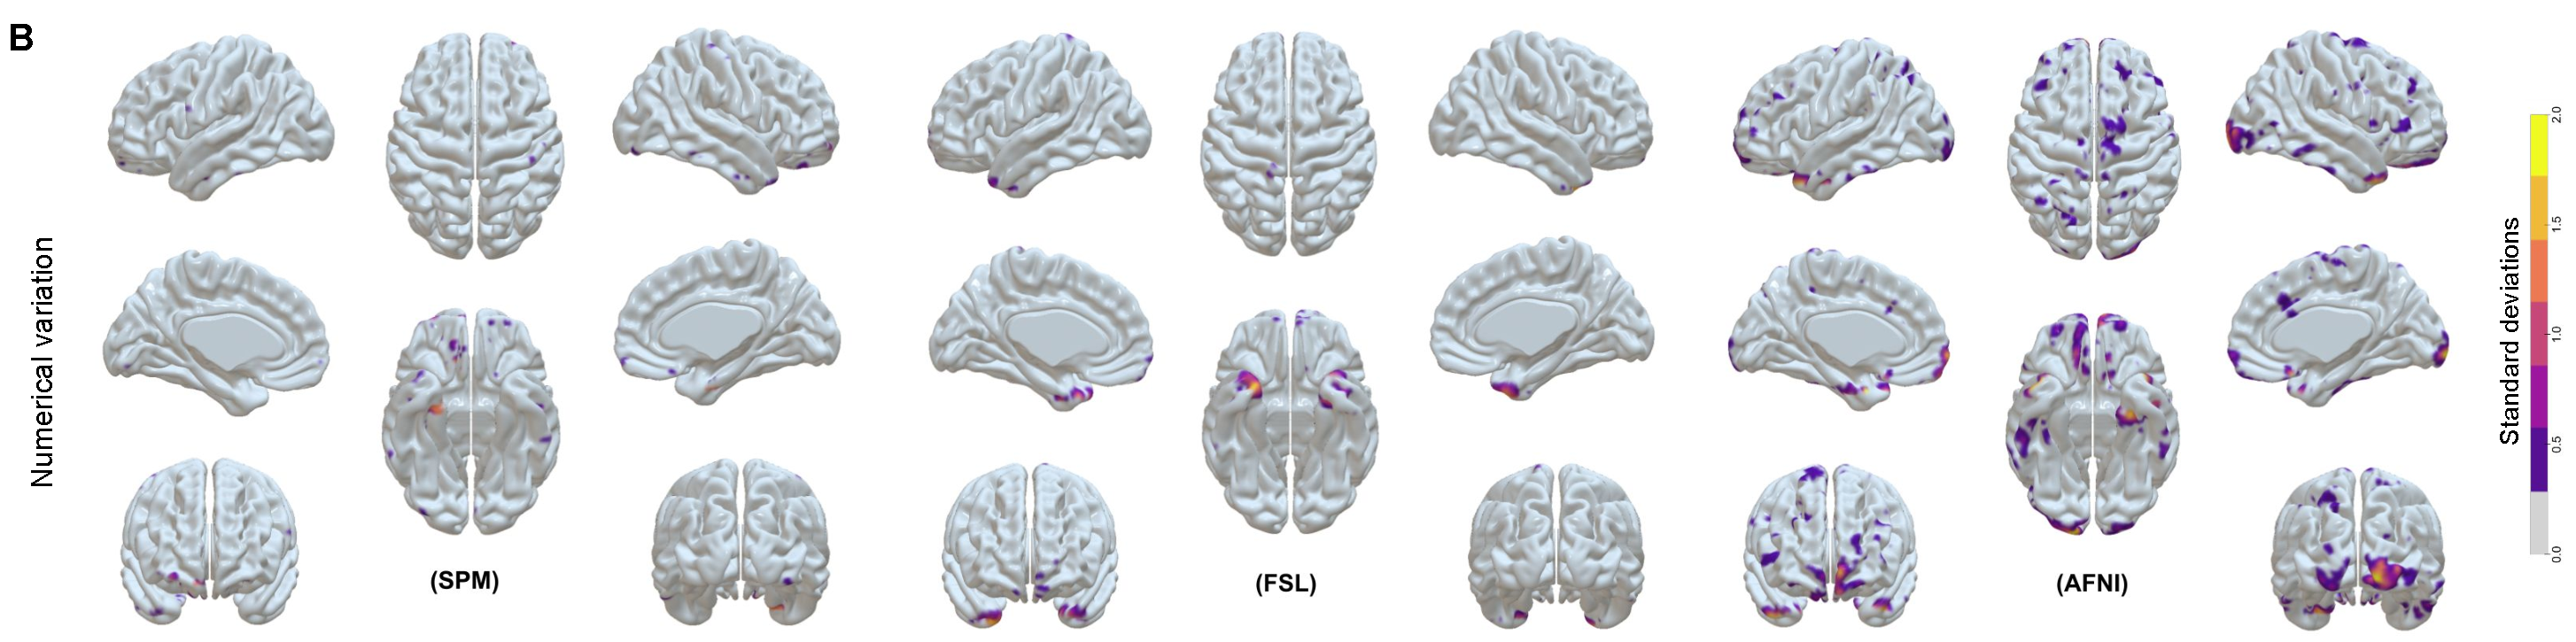
\includegraphics[width=\linewidth]{figures/maps-on-surf-unthresh-mca1(std).pdf}
    %\caption{Standard deviation of thresholded t-statistics map on template surface}
    \label{fig:thresh-stdmaps2}
  \end{subfigure}
  \caption{Surface maps of standard deviation of unthresholded t-statistics.}
  \label{fig:thresh-stdmaps}
  \end{minipage}}
\end{figure}


%%%%%%%%%% Bar plots of Dices from Thresh %%%%%%%%
\begin{figure}[b]
  \fbox{\begin{minipage}{\dimexpr \textwidth-2\fboxsep-2\fboxrule}

      \begin{subfigure}[t]{0.5\linewidth}
        \centering
        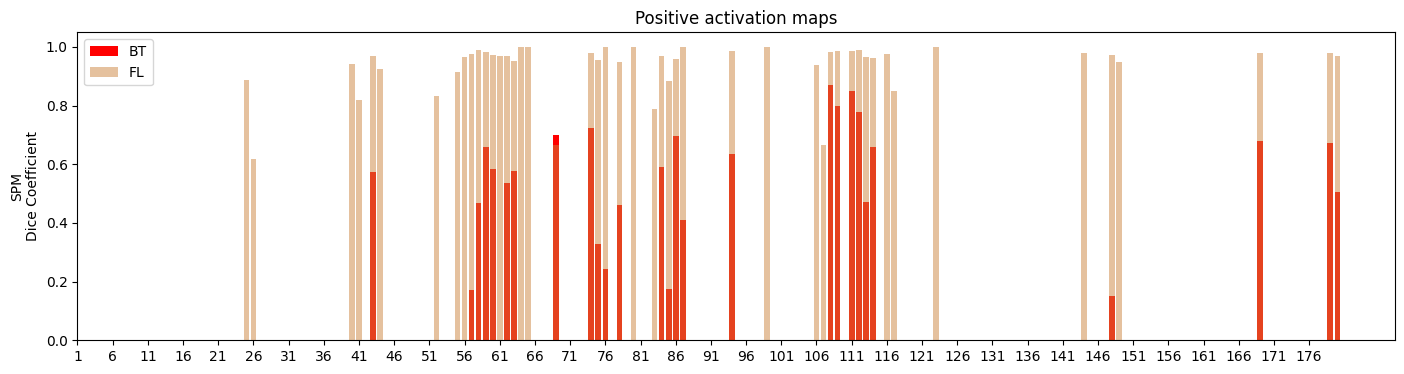
\includegraphics[width=\linewidth]{figures/spm-exc_set_file.png}
        \label{fig:fsl-dices}
      \end{subfigure}
      \hfill
      \begin{subfigure}[t]{0.5\linewidth}
        \centering
        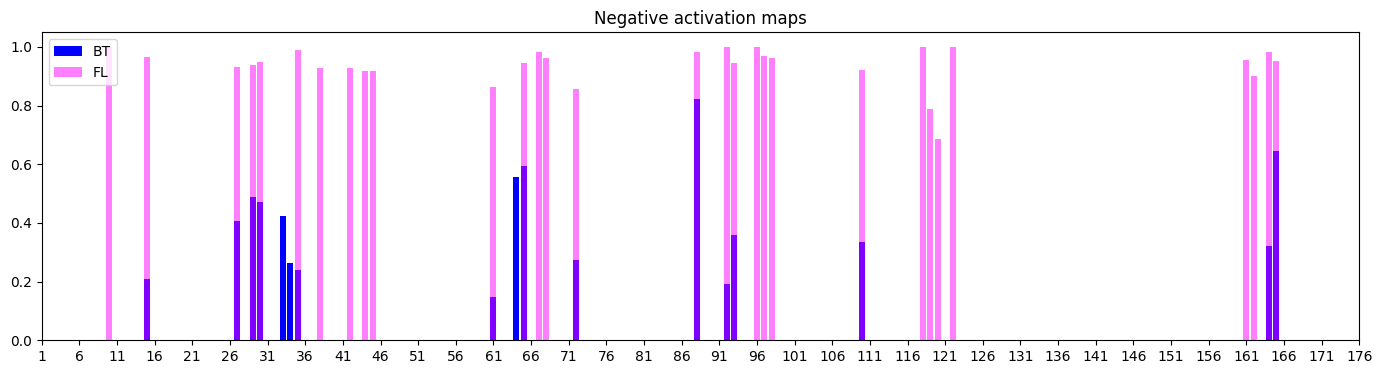
\includegraphics[width=\linewidth]{figures/spm-exc_set_file_neg.png}
        \label{fig:spm-dices}
      \end{subfigure}    
  \hfill
    \begin{subfigure}[t]{0.5\linewidth}
      \centering
      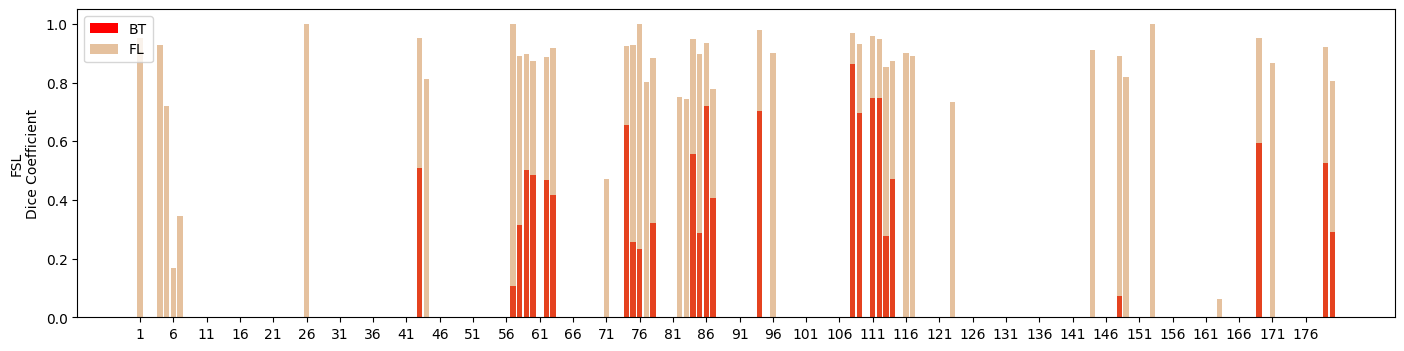
\includegraphics[width=\linewidth]{figures/fsl-exc_set_file.png}
      \label{fig:fsl-dices}
    \end{subfigure}
    \hfill
    \begin{subfigure}[t]{0.5\linewidth}
      \centering
      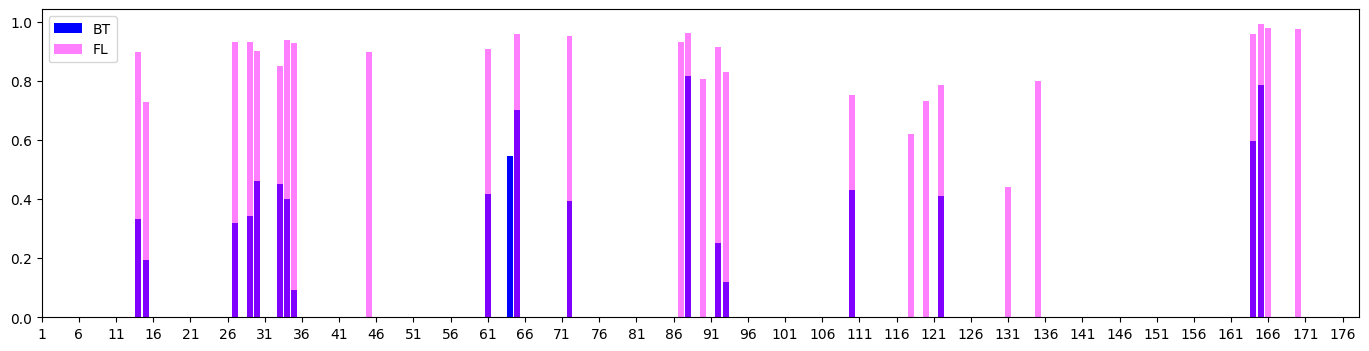
\includegraphics[width=\linewidth]{figures/fsl-exc_set_file_neg.png}
      \label{fig:spm-dices}
    \end{subfigure}  
  \hfill
    \begin{subfigure}[t]{0.5\linewidth}
      \centering
      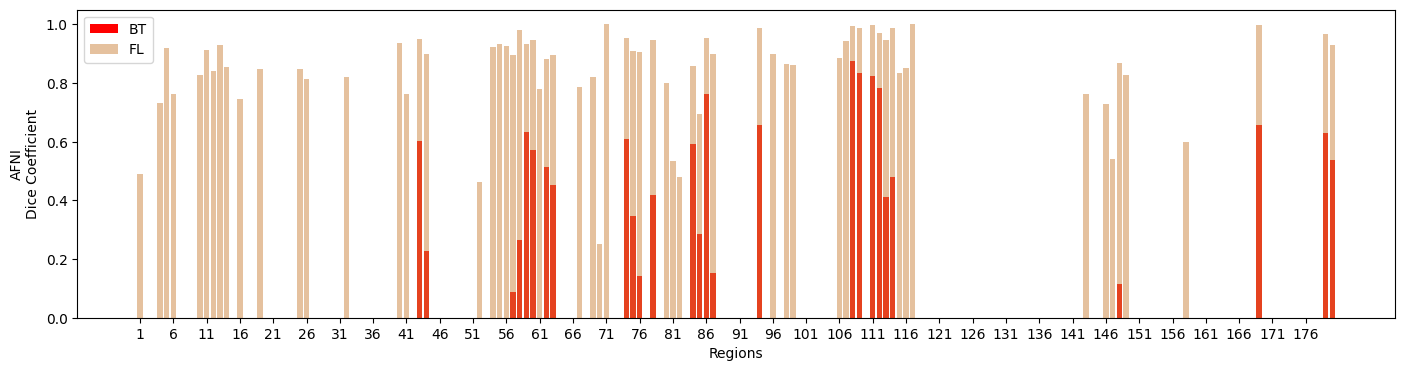
\includegraphics[width=\linewidth]{figures/afni-exc_set_file.png}
      \label{fig:fsl-dices}
    \end{subfigure}
    \hfill
    \begin{subfigure}[t]{0.5\linewidth}
      \centering
      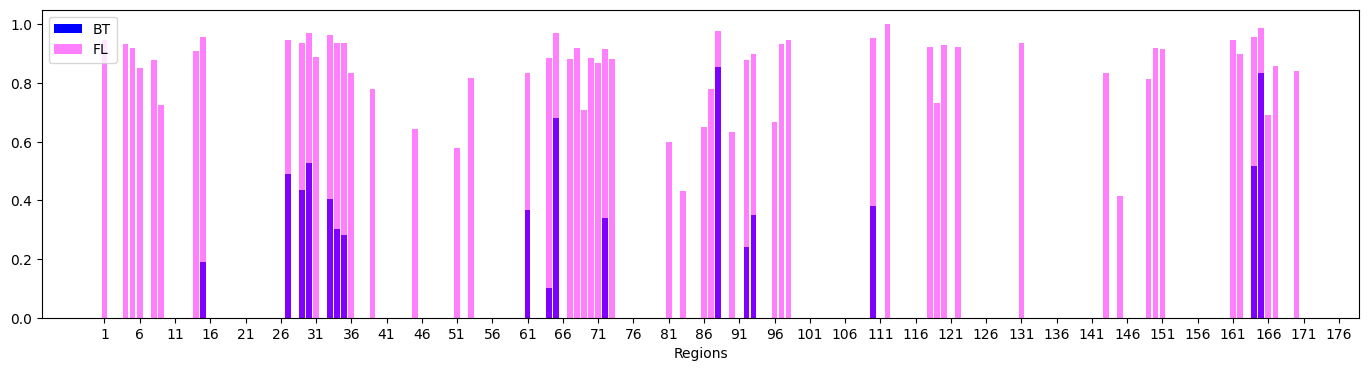
\includegraphics[width=\linewidth]{figures/afni-exc_set_file_neg.png}
      \label{fig:spm-dices}
    \end{subfigure}
  
  \caption{Bar plots of Dice coefficients of activated regions between pair of tools (BT) and fuzzy samples (FL) from the thresholded t-statistics.
  Right plots show the negative maps, and left plots show the positive maps. 
  Region numbers correspond to the 180 areas of cortical parcellation (HCP-MMP1.0)~\cite{Glasser-nature}.}
  \label{fig:unthresh-dices}
  \end{minipage}}
\end{figure}


%%%%%%%%%% Surf maps of Dices from Thresh %%%%%%%%
\begin{figure}[b]
  \fbox{\begin{minipage}{\dimexpr \textwidth-2\fboxsep-2\fboxrule}
  \begin{subfigure}[t]{\linewidth}
    \centering
    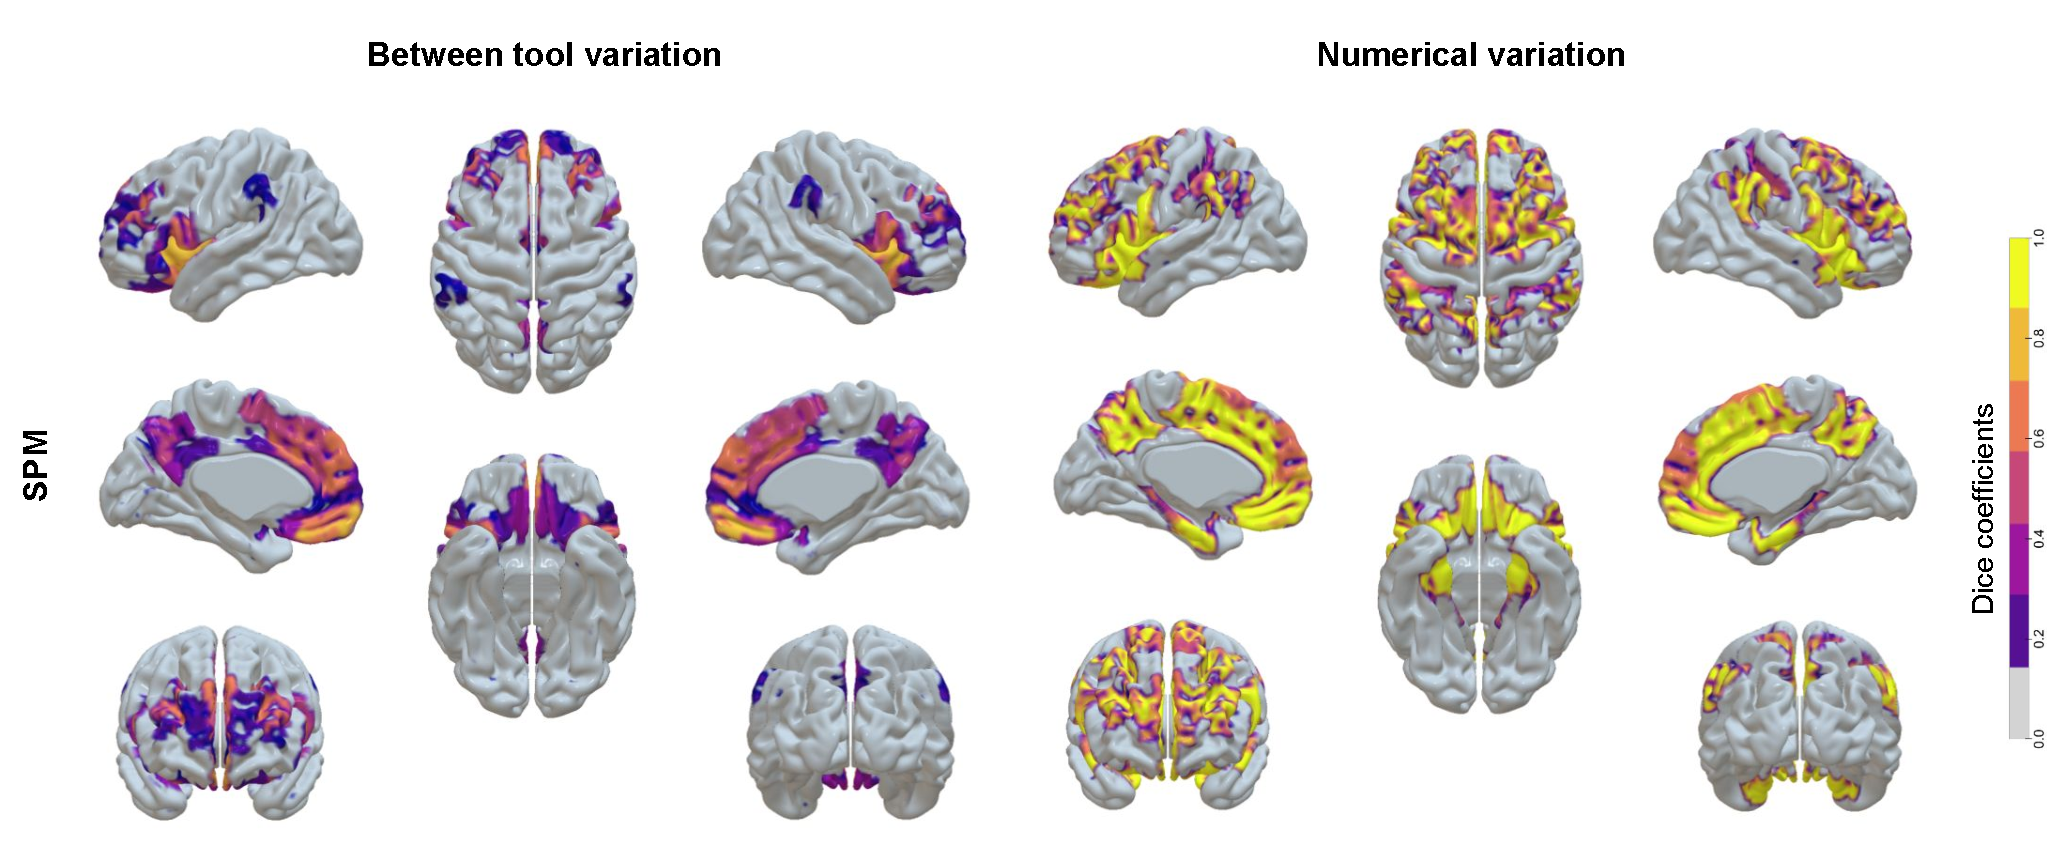
\includegraphics[width=\linewidth]{figures/maps-on-surf-SPM(dice).pdf}
    %\caption{Standard deviation of thresholded t-statistics map on template surface}
    \label{fig:thresh-stdmaps1}
  \end{subfigure}
  \hfill
  \begin{subfigure}[t]{\linewidth}
    \centering
    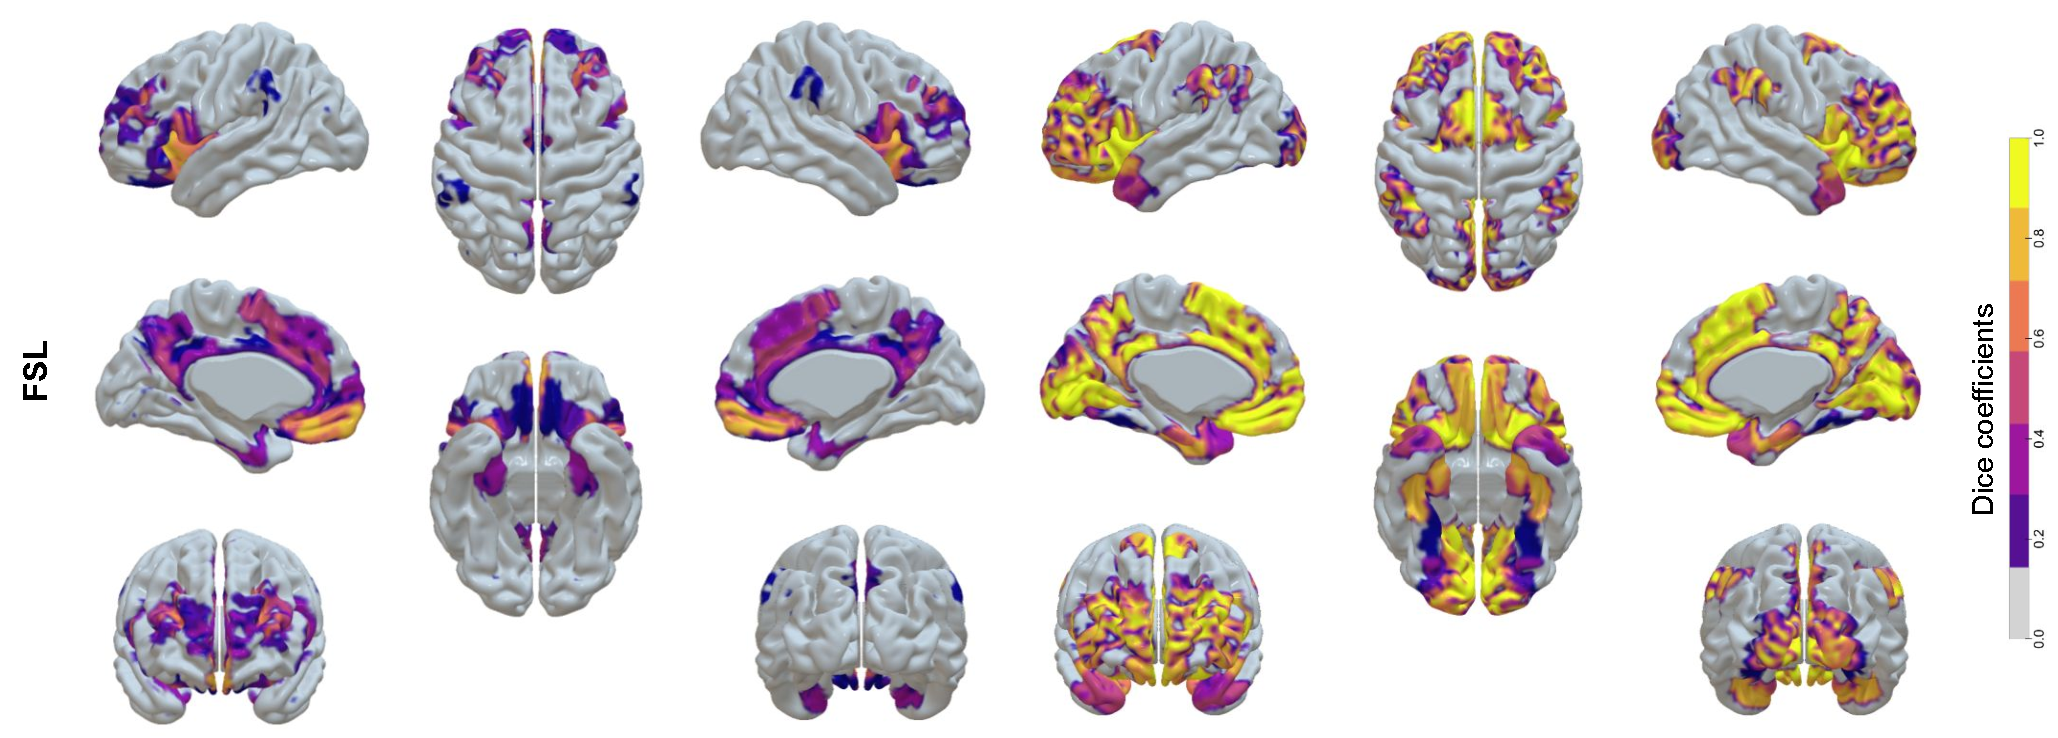
\includegraphics[width=\linewidth]{figures/maps-on-surf-FSL(dice).pdf}
    %\caption{Standard deviation of thresholded t-statistics map on template surface}
    \label{fig:thresh-stdmaps1}
  \end{subfigure}
  \hfill
  \begin{subfigure}[t]{\linewidth}
    \centering
    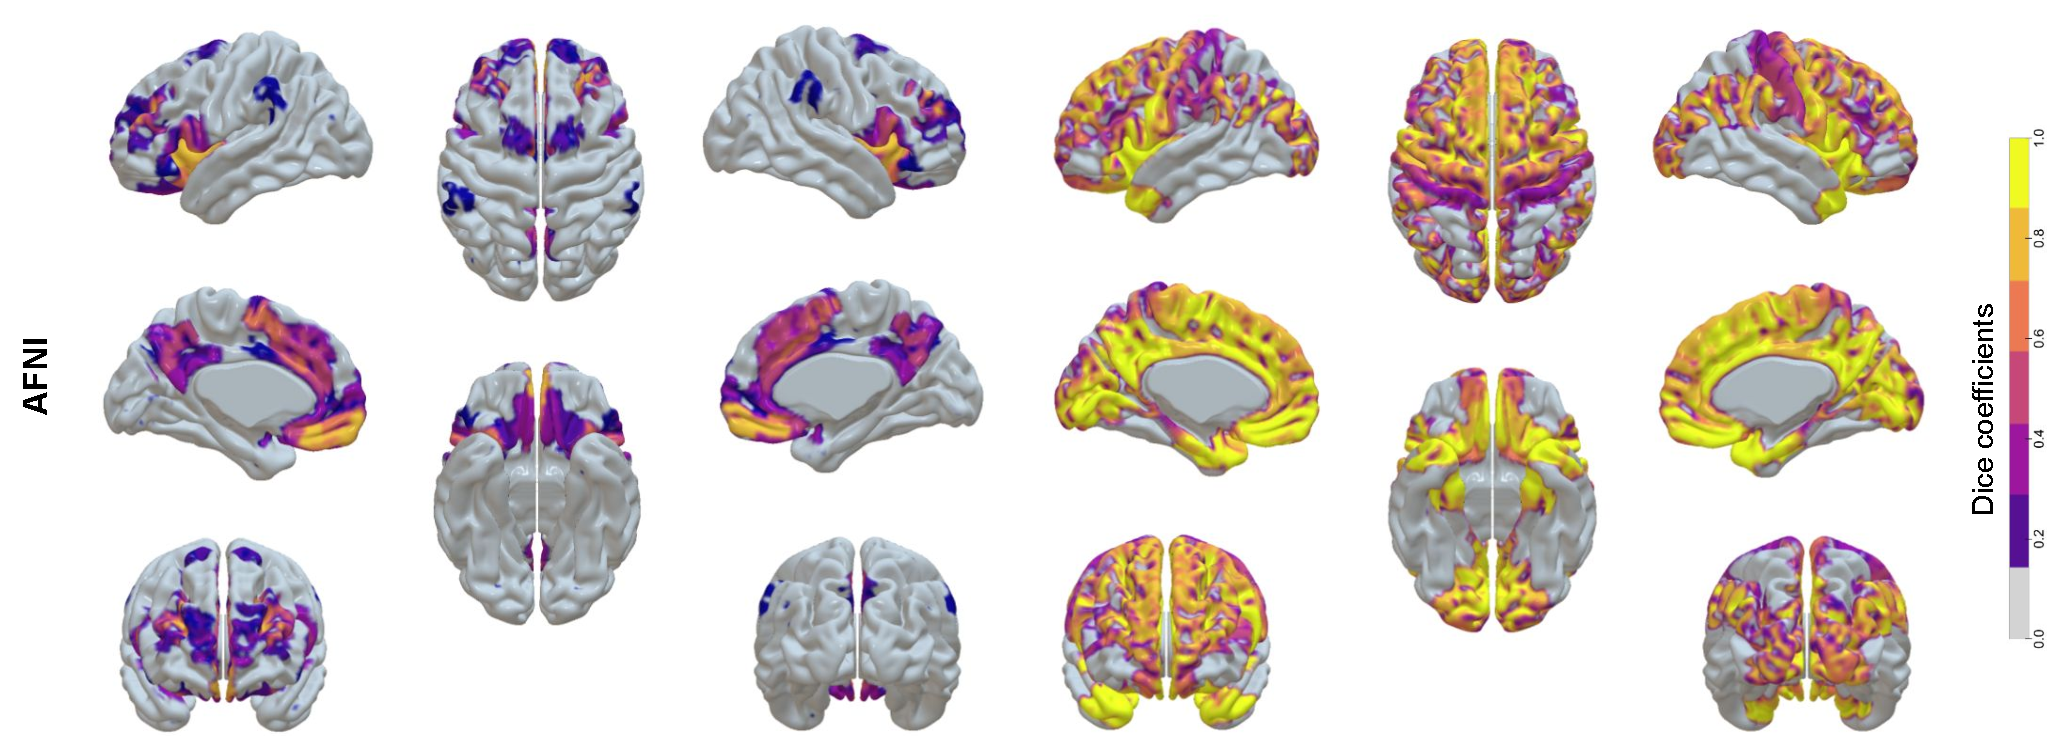
\includegraphics[width=\linewidth]{figures/maps-on-surf-AFNI(dice).pdf}
    %\caption{Standard deviation of thresholded t-statistics map on template surface}
    \label{fig:thresh-stdmaps2}
  \end{subfigure}
  \caption{Surface maps of Dice coefficients of thresholded t-statistics region-by-region.}
  \label{fig:unthresh-dices}
  \end{minipage}}
\end{figure}


% \subsection{The precision that Fuzzy FSL tool can simulate the between tool variations}
% \begin{description}
%   \item[$\bullet$ Figure 5:] Repeat Fig 1-4 for the results of Fuzzy FSL on the precision that simulate mostly betwen tool varions.
% \end{description}


\section{Conclusion \& Discussion}
conclusions\dots
%
% ---- Bibliography ----
%
% BibTeX users should specify bibliography style 'splncs04'.
% References will then be sorted and formatted in the correct style.
%
\bibliographystyle{splncs04}
\bibliography{biblio}

\end{document}
